%!TEX root = ../report.tex

% 
% Architecture
% 

\section{Architecture}
\label{sec:architecture}
This section is about the project's architecture.
Our solution is split in two main components.
The Smart Places App is an Android app that the user
would have to install and that will give him access
to any app running in any Smart Place. Also, any
Smart Place owner could use this app to install
apps in his space.
The framework would allow developers to develop their
proximity-based apps for Smart Spaces without writing
the code to get the beacons' signals and get the data
from a back-end. 
% 2/3 pages
%Your proposed architecture. Can have lots of pictures and 
% bullet points so it is easy to understand.
\begin{figure}[!ht]
  \caption{Architecture}
  \label{fig:architecture}
  \centering
    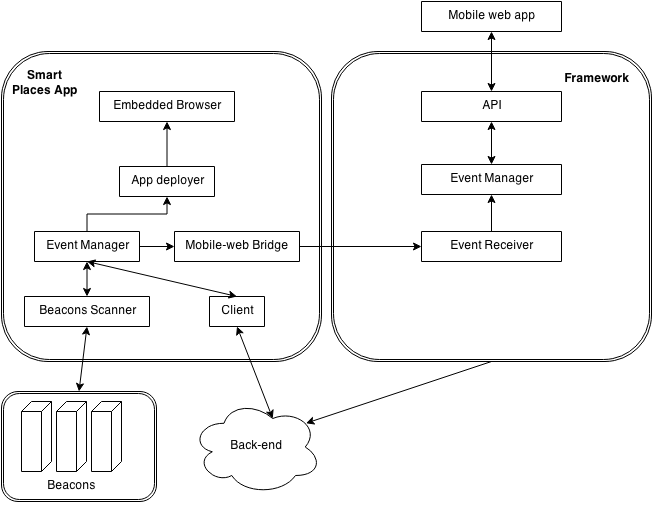
\includegraphics[width=0.9\textwidth]{img/architecture}
\end{figure}

\subsection{Smart Places App}
\label{sub:smart_places_app}
\textbf{Beacons Scanner:} 
Scans for beacons and get their IDs.
\\
\textbf{Client:} 
Communicates with the back-end
\\
\textbf{Event Manager:} 
Gets scanned beacons data and send that to the client.
The Client will send a request to the back-end to get the
information associated to the scanned beacons
\\
\textbf{App Deployer:} 
After getting the POI information represented by a given beacon,
it will send the corresponding mobile web app in the Embedded
Browser
\\
\textbf{Embedded Browser:} 
Shows the mobile web apps to the user in a embedded web browser
in the Smart Places App
\\
\textbf{Mobile-Web Bridge:} 
Receives events from the Event Manager, such as, the user
is nearby a given POI and sent those events to the Event Receiver,
that runs in the mobile web app.
\\

\subsection{Framework}
\label{sub:framework}
\textbf{Event Receiver:} 
Receives events from the Mobile-Web Bridge,
that runs in the Smart Places App and sends them to the
Event Manager
\\
\textbf{Event Manager:} 
Receives events from the Event Receiver and handles them, using
handlers defined by the developer of the mobile web app.
\\
\textbf{API:} 
Application Programming Interface, available to developers, to 
allow them to set the behavior of each POI
\\
